\documentclass[conference]{IEEEtran}
\IEEEoverridecommandlockouts
\usepackage{amsmath,amssymb,amsfonts}
\usepackage{algorithmic}
\usepackage{graphicx}
\usepackage{textcomp}
\usepackage{xcolor}

\usepackage{calc}
\usepackage{enumitem}
\usepackage{xspace}

\usepackage{url}

\usepackage[numbers,square,sort&compress]{natbib}
\usepackage{balance}


\usepackage{booktabs}
\usepackage{tabularx}
\usepackage{multirow}

\usepackage{microtype}


\renewcommand{\paragraph}[1]{{\vskip 8pt \noindent\bf #1 }}


\newcommand{\srcimg}{\ensuremath{S}\xspace}
\newcommand{\tarimg}{\ensuremath{T}\xspace}
\newcommand{\attimg}{\ensuremath{A}\xspace}
\newcommand{\outimg}{\ensuremath{D}\xspace}
\newcommand{\deltaS}{\ensuremath{\Delta}\xspace}
\newcommand{\scalefunc}{\ensuremath{\mathrm{scale}}}

\newcommand{\ti}{\ensuremath{Z}\xspace}



\newcommand{\goalA}{O1\xspace} %
\newcommand{\goalB}{O2\xspace} %


\definecolor{goeblue}{RGB}{0,51,102}
\definecolor{denceblue}{RGB}{6,107,176}
\definecolor{sunygreen}{RGB}{0,166,77}
\definecolor{darkgreentone}{RGB}{60,179,113}
\definecolor{tubsredSec}{cmyk}{0.0,1.00,0.6,0.6}
\definecolor{tubsredPrim}{cmyk}{0.1,1.0,0.8,0.0}
\newcommand{\head}[1]{\textnormal{\textbf{#1}}}



\def\BibTeX{{\rm B\kern-.05em{\sc i\kern-.025em b}\kern-.08em
    T\kern-.1667em\lower.7ex\hbox{E}\kern-.125emX}}
\begin{document}

\title{Backdooring and Poisoning Neural Networks\\with 
	Image-Scaling Attacks\thanks{Published at {IEEE} Deep Learning and
		Security Workshop (DLS) 2020, co-located with the 41st {IEEE} 
		Symposium on Security and Privacy (S\&P)}}

\author{
	{\rm Erwin Quiring and 
		Konrad Rieck}\\[1mm]
	\begin{minipage}{8cm} 
		\centering \it
		Technische Universit\"at Braunschweig, Germany
	\end{minipage} 	  %
}

\maketitle



\begin{abstract}
Backdoors and poisoning attacks are a major threat to the security of 
machine-learning and vision systems. Often, however, these attacks 
leave visible artifacts in the images that can be visually detected and 
weaken the efficacy of the attacks.  In this paper, we propose a novel 
strategy for hiding backdoor and poisoning attacks. Our approach builds 
on a recent class of attacks against image scaling. These attacks 
enable manipulating images such that they change their content when 
scaled to a specific resolution. By combining poisoning and 
image-scaling attacks, we can conceal the trigger of backdoors as well 
as hide the overlays of clean-label poisoning. Furthermore, we consider 
the detection of image-scaling attacks and derive an adaptive attack. 
In an empirical evaluation, we demonstrate the effectiveness of our 
strategy.  First, we show that backdoors and poisoning work equally 
well when combined with image-scaling attacks. Second, we demonstrate 
that current detection defenses against image-scaling attacks are 
insufficient to uncover our manipulations. Overall, our work provides a 
novel means for hiding traces of manipulations, being applicable to 
different poisoning approaches.
\end{abstract}

\vspace{0.2cm}

\section{Introduction}
Machine Learning is nowadays used in various security-critical 
applications that range from intrusion detection and medical 
systems to autonomous cars. Despite remarkable results, 
research on the security of machine learning has revealed various 
possible attacks.
A considerable threat are poisoning attacks during the training 
process~\citep[e.g.][]{BigNelLas11, GuDolGar17, LiuMaAaf+18}. 
Deep learning applications usually require a large number of 
training instances, so that there is a risk of an insider carefully 
manipulating a portion of the training data. Moreover, the training 
process can be outsourced either due to a lack of expertise in deep 
learning or due to missing computational resources to train large 
networks---again giving the chance to manipulate training data and the 
model.

In the context of deep learning, recent research has demonstrated that 
neural networks can be modified to return targeted responses without an 
impact on their behavior for benign inputs. An adversary, for instance, 
can insert a pattern in some training images of a particular 
target class, so that the network learns to associate the pattern with 
this class. If the pattern is added to arbitrary images, the network 
returns the target class.
However, a major drawback of most attacks is the visibility of data 
manipulations either at training or test time~\citep{GuDolGar17, 
LiuMaAaf+18}. The attack is thus revealed if human beings 
audit the respective images. 

\citet{XiaCheShe+19} have recently presented a novel attack 
vulnerability in the data preprocessing of typical machine learning 
pipelines. An adversary can slightly manipulate an image, such that an
\emph{image scaling} algorithm produces a novel and unrelated image in 
the network's input dimensions. The attack exploits that images are 
typically larger than the input dimensions and thus need to be scaled.

This novel attack directly addresses the shortcomings of 
most poisoning attacks by allowing an adversary to conceal data 
manipulations. As an example, Figure~\ref{fig:intro_example_poisoning} 
shows a clean-label poisoning attack~\citep{ShaHuaNaj+18} on the 
popular TensorFlow library. The network will learn to classify 
the dog as cat if this dog is repeatedly inserted into 
varying images showing cats during training.
In the attack's standard version, the slight manipulation of the 
training image is still noticeable. Yet, image-scaling attacks conceal 
the manipulation of the training data effectively. The dog appears only 
in the downscaled image which is finally used by the neural network.



\begin{figure}[t]
	\centering
	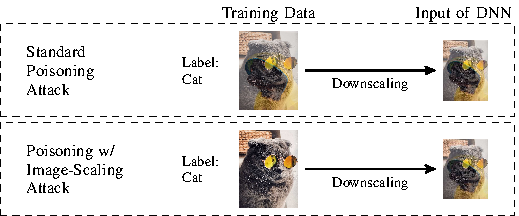
\includegraphics{./ext_images/scaler_poisoning-figure0.pdf}
	\vspace{-0.59cm}
	\caption{Example of a clean-label poisoning 
	attack~\citep{ShaHuaNaj+18}: a neural network 
	learns to classify a dog as cat by blending the dog with multiple 
	cat images. %
	Image-scaling attacks allow more insidious poisoning attacks.
	The dog as manipulation is not visible in the training data and 
	appears only after downscaling.
	}
	\label{fig:intro_example_poisoning}
\end{figure}

This paper provides the first analysis on the combination of data 
poisoning and image-scaling attacks. Our findings show that an 
adversary can significantly conceal image manipulations of current 
backdoor attacks~\citep{GuDolGar17} and clean-label 
attacks~\citep{ShaHuaNaj+18} without an impact on their overall attack 
success rate.
Moreover, we demonstrate that defenses---designed to detect 
image-scaling attacks---fail in the poisoning scenario.
We examine the histogram- and color-scattering-based detection as 
proposed by~\citet{XiaCheShe+19}. In an empirical evaluation, we show 
that both defenses cannot detect backdoor attacks due to bounded, 
local changes. We further derive a novel adaptive attack that 
significantly reduces the performance of both defenses in the 
clean-label setting.
All in all, our findings indicate a need for novel, robust detection 
defenses against image-scaling~attacks.
\paragraph{Contributions.}  In summary, we make the following
contributions in this paper:
\begin{itemize}  \setlength{\itemsep}{3pt}
	
	\item \emph{Combination of data poisoning and image-scaling 
	attacks.}  
	We provide the first analysis on poisoning attacks that are 
	combined with image-scaling attacks. We discuss two realistic 
	threat models and consider backdoor attacks as well as clean-label 
	poisoning attacks.
		
	\item \emph{Evaluation of defenses} 
	We evaluate current detection methods against image-scaling 
	attacks and show that backdoor attacks cannot be detected.
	
	\item \emph{Adaptive Attack.} We derive a novel variant of
	image-scaling attack that reduces the detection rate 
	of current scaling defenses. Our evaluation 
	shows that clean-label attacks cannot be reliably detected anymore.
\end{itemize}

The remainder of this paper is organized as follows: 
Section~\ref{sec:background} reviews the background of data poisoning 
and image-scaling attacks. Section~\ref{sec:poisoning-scaling} examines 
their combination with the respective threat scenarios and our adaptive 
attack.
Section~\ref{sec:eval} provides an empirical evaluation of attacks and 
defenses.
Section~\ref{sec:limitations} and~\ref{sec:relatedwork} present 
limitations and related work, respectively. 
Section~\ref{sec:conclusion} concludes the paper.



\section{Background}\label{sec:background}
Let us start by briefly examining poisoning and image-scaling 
attacks on machine learning. Both attacks operate at different stages 
in a typical machine learning pipeline and allow more powerful attacks 
when combined, as we will show in the remainder of this work.

 
\section{Related Work}\label{sec:relatedwork}
The secure application of machine learning requires considering 
various attacks along a typical workflow. 
Regarding the order of the targeted step, attacks can be
categorized into the following classes:
membership inference~\citep[e.g.,][]{ShoStrSonShm17}, poisoning 
attacks~\citep[e.g.,][]{BigNelLas11, GuDolGar17, LiuMaAaf+18}, 
evasion- and perturbation
attacks~\citep[e.g.,][]{BigCorMai+13,CarWag17,QuiMaiRie19}, as
well as model stealing~\citep[e.g.,][]{TraZhaJuel+16}.

In this work, we focus on poisoning attacks that manipulate the 
training data so that the learning model returns targeted 
responses with adversarial inputs only while behaving normally for 
benign inputs. Two attack variants are backdoor and clean-label 
poisoning attacks, differing in the the amount of necessary data 
changes, visibility or robustness with transfer 
learning~\citep[e.g.][]{GuDolGar17, CheLiuLi+17, ShaHuaNaj+18, 
LiuMaAaf+18, YaoLiZhe+19}. 
We consider the following two rather simple, but representative 
approaches:
The BadNets method~\citep{GuDolGar17} inserts a small, bounded pattern 
into images as backdoor, while the clean-label attack 
from~\citet{ShaHuaNaj+18} slightly changes the whole image to add a 
poison. Both provide first insights about the 
applicability of image-scaling attacks for data poisoning.

Concurrently, \citet{QuiKleArp20} comprehensively analyze 
image-scaling attacks by identifying the root-cause and examining
defenses for \emph{prevention}. Our work here extends this line of 
research on image-scaling attacks by analyzing the poisoning 
application and \emph{detection} defenses.  While prevention stops any 
attack, detection uncovers that an attack is going on. Our findings 
here underline the need for novel detection~approaches.




\section{Conclusion}\label{sec:conclusion}
This work demonstrates that image-scaling attacks can be 
leveraged to hide data manipulations for poisoning attacks. We consider 
two representative approaches: a backdoor attack~\citep{GuDolGar17} and 
a clean-label poisoning attack~\citep{ShaHuaNaj+18}. Our evaluation 
shows that the adversary can conceal manipulations more effectively 
without impact on the overall success rate of her poisoning attack. 
We find that image-scaling attacks can create almost invisible poisoned 
instances if a slight manipulation is spread over a larger area of the 
input.


Furthermore, our work raises the need for novel detection defenses 
against image-scaling attacks. Local and bounded changes---as done for 
backdoors---are not detected at all. The detection if the whole image 
is changed can be circumvented by using our proposed adaptive 
image-scaling attack variant. 


\footnotesize{
\bibliographystyle{abbrvnat}
\balance

\begin{thebibliography}{21}
	\providecommand{\natexlab}[1]{#1}
	\providecommand{\url}[1]{\texttt{#1}}
	\expandafter\ifx\csname urlstyle\endcsname\relax
	\providecommand{\doi}[1]{doi: #1}\else
	\providecommand{\doi}{doi: \begingroup \urlstyle{rm}\Url}\fi
	
	\bibitem[Biggio et~al.(2011)Biggio, Nelson, and Laskov]{BigNelLas11}
	B.~Biggio, B.~Nelson, and P.~Laskov.
	\newblock Support vector machines under adversarial label noise.
	\newblock In \emph{Proc. of Asian Conference on Machine Learning 
	{(ACML)}},
	pages 97--112, 2011.
	
	\bibitem[Biggio et~al.(2013)Biggio, Corona, Maiorca, Nelson,
	{\v{S}}rndi{\'{c}}, Laskov, Giacinto, and Roli]{BigCorMai+13}
	B.~Biggio, I.~Corona, D.~Maiorca, B.~Nelson, N.~{\v{S}}rndi{\'{c}}, 
	P.~Laskov,
	G.~Giacinto, and F.~Roli.
	\newblock Evasion attacks against machine learning at test time.
	\newblock In \emph{Machine Learning and Knowledge Discovery in 
	Databases},
	pages 387--402. Springer, 2013.
	
	\bibitem[Carlini and Wagner(2017)]{CarWag17}
	N.~Carlini and D.~A. Wagner.
	\newblock Towards evaluating the robustness of neural networks.
	\newblock In \emph{Proc. of {IEEE} Symposium on Security and 
	Privacy ({S\&P})},
	2017.
	
	\bibitem[Chen et~al.(2017)Chen, Liu, Li, Lu, and Song]{CheLiuLi+17}
	X.~Chen, C.~Liu, B.~Li, K.~Lu, and D.~Song.
	\newblock Targeted backdoor attacks on deep learning systems using 
	data
	poisoning.
	\newblock Technical report, arXiv:1712.05526, 2017.
	
	\bibitem[Gu et~al.(2017)Gu, Dolan{-}Gavitt, and Garg]{GuDolGar17}
	T.~Gu, B.~Dolan{-}Gavitt, and S.~Garg.
	\newblock Badnets: Identifying vulnerabilities in the machine 
	learning model
	supply chain.
	\newblock Technical report, arXiv:1708.06733, 2017.
	
	\bibitem[Kloft and Laskov(2010)]{KloLas10a}
	M.~Kloft and P.~Laskov.
	\newblock Online anomaly detection under adversarial impact.
	\newblock In \emph{JMLR Workshop and Conference Proceedings, Volume 
	9:
		AISTATS}, pages 405--412, 2010.
	
	\bibitem[Krizhevsky et~al.(2009)Krizhevsky, Hinton, 
	et~al.]{KriHin09}
	A.~Krizhevsky, G.~Hinton, et~al.
	\newblock Learning multiple layers of features from tiny images.
	\newblock Technical report, 2009.
	
	\bibitem[Liu et~al.(2018)Liu, Ma, Aafer, Lee, Zhai, Wang, and
	Zhang]{LiuMaAaf+18}
	Y.~Liu, S.~Ma, Y.~Aafer, W.-C. Lee, J.~Zhai, W.~Wang, and X.~Zhang.
	\newblock Trojaning attack on neural networks.
	\newblock In \emph{Proc. of Network and Distributed System Security 
	Symposium
		({NDSS})}, 2018.
	
	\bibitem[Quiring et~al.(2019)Quiring, Maier, and Rieck]{QuiMaiRie19}
	E.~Quiring, A.~Maier, and K.~Rieck.
	\newblock Misleading authorship attribution of source code using 
	adversarial
	learning.
	\newblock In \emph{Proc. of {USENIX} Security Symposium}, pages 
	479--496, 2019.
	
	\bibitem[Quiring et~al.(2020)Quiring, Klein, Arp, Johns, and
	Rieck]{QuiKleArp20}
	E.~Quiring, D.~Klein, D.~Arp, M.~Johns, and K.~Rieck.
	\newblock Adversarial preprocessing: Understanding and preventing 
	image-scaling
	attacks in machine learning.
	\newblock In \emph{Proc. of USENIX Security Symposium}, 2020.
	
	\bibitem[Russakovsky et~al.(2015)Russakovsky, Deng, Su, Krause, 
	Satheesh, Ma,
	Huang, Karpathy, Khosla, Bernstein, Berg, and Fei-Fei]{RusDenSu+15}
	O.~Russakovsky, J.~Deng, H.~Su, J.~Krause, S.~Satheesh, S.~Ma, 
	Z.~Huang,
	A.~Karpathy, A.~Khosla, M.~Bernstein, A.~C. Berg, and L.~Fei-Fei.
	\newblock {ImageNet Large Scale Visual Recognition Challenge}.
	\newblock \emph{International Journal of Computer Vision (IJCV)}, 
	115\penalty0
	(3):\penalty0 211--252, 2015.
	
	\bibitem[Shafahi et~al.(2018)Shafahi, Huang, Najibi, Suciu, Studer, 
	Dumitras,
	and Goldstein]{ShaHuaNaj+18}
	A.~Shafahi, W.~R. Huang, M.~Najibi, O.~Suciu, C.~Studer, 
	T.~Dumitras, and
	T.~Goldstein.
	\newblock Poison frogs! {T}argeted clean-label poisoning attacks on 
	neural
	networks.
	\newblock In \emph{Advances in Neural Information Processing 
	Systems ({NIPS})},
	pages 6103--6113, 2018.
	
	\bibitem[Shokri et~al.(2017)Shokri, Stronati, Song, and
	Shmatikov]{ShoStrSonShm17}
	R.~Shokri, M.~Stronati, C.~Song, and V.~Shmatikov.
	\newblock Membership inference attacks against machine learning 
	models.
	\newblock In \emph{Proc. of {IEEE} Symposium on Security and 
	Privacy ({S\&P})},
	2017.
	
	\bibitem[Simonyan and Zisserman(2014)]{SimZis14}
	K.~Simonyan and A.~Zisserman.
	\newblock Very deep convolutional networks for large-scale image 
	recognition.
	\newblock Technical report, arXiv:1409.1556, 2014.
	
	\bibitem[Stoneff(2015)]{Sto15}
	C.~Stoneff.
	\newblock The insider versus the outsider: Who poses the biggest 
	security risk?
	\newblock
	\url{https://www.helpnetsecurity.com/2015/08/19/the-insider-versus-the-outsider-who-poses-the-biggest-security-risk/},
	2015.
	\newblock Accessed: 2020-01-07.
	
	\bibitem[Szegedy et~al.(2015)Szegedy, Vanhoucke, Ioffe, Shlens, and
	Wojna]{SzeVanIof+15}
	C.~Szegedy, V.~Vanhoucke, S.~Ioffe, J.~Shlens, and Z.~Wojna.
	\newblock Rethinking the inception architecture for computer vision.
	\newblock In \emph{IEEE Conference on Computer Vision and Pattern 
	Recognition
		(CVPR)}, pages 2818--2826, 2015.
	
	\bibitem[Tan and Shokri(2019)]{TanSho19}
	T.~J.~L. Tan and R.~Shokri.
	\newblock Bypassing backdoor detection algorithms in deep learning.
	\newblock Technical report, arXiv:1905.13409, 2019.
	
	\bibitem[Tram{\`e}r et~al.(2016)Tram{\`e}r, Zhang, Juels, Reiter, 
	and
	Ristenpart]{TraZhaJuel+16}
	F.~Tram{\`e}r, F.~Zhang, A.~Juels, M.~K. Reiter, and T.~Ristenpart.
	\newblock Stealing machine learning models via prediction apis.
	\newblock In \emph{Proc. of {USENIX} Security Symposium}, pages 
	601--618, 2016.
	
	\bibitem[Wang et~al.(2019)Wang, Yao, Shan, Li, Viswanath, Zheng, and
	Zhao]{WanYaoShaLi+19}
	B.~Wang, Y.~Yao, S.~Shan, H.~Li, B.~Viswanath, H.~Zheng, and B.~Y. 
	Zhao.
	\newblock Neural cleanse: Identifying and mitigating backdoor 
	attacks in neural
	networks.
	\newblock In \emph{Proc. of {IEEE} Symposium on Security and 
	Privacy ({S\&P})},
	pages 707--723, 2019.
	
	\bibitem[Xiao et~al.(2019)Xiao, Chen, Shen, Chen, and 
	Li]{XiaCheShe+19}
	Q.~Xiao, Y.~Chen, C.~Shen, Y.~Chen, and K.~Li.
	\newblock Seeing is not believing: Camouflage attacks on image 
	scaling
	algorithms.
	\newblock In \emph{Proc. of {USENIX} Security Symposium}, pages 
	443--460, 2019.
	
	\bibitem[Yao et~al.(2019)Yao, Li, Zheng, and Zhao]{YaoLiZhe+19}
	Y.~Yao, H.~Li, H.~Zheng, and B.~Y. Zhao.
	\newblock Latent backdoor attacks on deep neural networks.
	\newblock In \emph{Proc. of {ACM} Conference on Computer and 
	Communications
		Security ({CCS})}, pages 2041–--2055, 2019.
	
\end{thebibliography}

}


\end{document}
